\documentclass[journal,12pt,twocolumn]{IEEEtran}
\usepackage{setspace}
\usepackage{gensymb}
\singlespacing
\usepackage[cmex10]{amsmath}
\usepackage{amsthm}
\usepackage{mathrsfs}
\usepackage{txfonts}
\usepackage{stfloats}
\usepackage{bm}
\usepackage{cite}
\usepackage{cases}
\usepackage{subfig}
\usepackage{longtable}
\usepackage{multirow}
\usepackage{enumitem}
\usepackage{mathtools}
\usepackage{tikz}
\usepackage{circuitikz}
\usepackage{verbatim}
\usepackage[breaklinks=true]{hyperref}
\usepackage{tkz-euclide} % loads  TikZ and tkz-base
\usepackage{listings}
\usepackage{color}    
\usepackage{array}    
\usepackage{longtable}
\usepackage{calc}     
\usepackage{multirow} 
\usepackage{hhline}   
\usepackage{ifthen}   
\usepackage{lscape}     
\usepackage{chngcntr}
\DeclareMathOperator*{\Res}{Res}
\renewcommand\thesection{\arabic{section}}
\renewcommand\thesubsection{\thesection.\arabic{subsection}}
\renewcommand\thesubsubsection{\thesubsection.\arabic{subsubsection}}

\renewcommand\thesectiondis{\arabic{section}}
\renewcommand\thesubsectiondis{\thesectiondis.\arabic{subsection}}
\renewcommand\thesubsubsectiondis{\thesubsectiondis.\arabic{subsubsection}}
\renewcommand\thetable{\arabic{table}}
% correct bad hyphenation here
\hyphenation{op-tical net-works semi-conduc-tor}
\def\inputGnumericTable{}                                 %%

\lstset{
%language=C,
frame=single, 
breaklines=true,
columns=fullflexible
}
%\lstset{
%language=tex,
%frame=single, 
%breaklines=true
%}

\begin{document}
\newtheorem{theorem}{Theorem}[section]
\newtheorem{problem}{Problem}
\newtheorem{proposition}{Proposition}[section]
\newtheorem{lemma}{Lemma}[section]
\newtheorem{corollary}[theorem]{Corollary}
\newtheorem{example}{Example}[section]
\newtheorem{definition}[problem]{Definition}
\newcommand{\BEQA}{\begin{eqnarray}}
\newcommand{\EEQA}{\end{eqnarray}}
\newcommand{\define}{\stackrel{\triangle}{=}}
\bibliographystyle{IEEEtran}
\providecommand{\mbf}{\mathbf}
\providecommand{\pr}[1]{\ensuremath{\Pr\left(#1\right)}}
\providecommand{\qfunc}[1]{\ensuremath{Q\left(#1\right)}}
\providecommand{\sbrak}[1]{\ensuremath{{}\left[#1\right]}}
\providecommand{\lsbrak}[1]{\ensuremath{{}\left[#1\right.}}
\providecommand{\rsbrak}[1]{\ensuremath{{}\left.#1\right]}}
\providecommand{\brak}[1]{\ensuremath{\left(#1\right)}}
\providecommand{\lbrak}[1]{\ensuremath{\left(#1\right.}}
\providecommand{\rbrak}[1]{\ensuremath{\left.#1\right)}}
\providecommand{\cbrak}[1]{\ensuremath{\left\{#1\right\}}}
\providecommand{\lcbrak}[1]{\ensuremath{\left\{#1\right.}}
\providecommand{\rcbrak}[1]{\ensuremath{\left.#1\right\}}}
\theoremstyle{remark}
\newtheorem{rem}{Remark}
\newcommand{\sgn}{\mathop{\mathrm{sgn}}}
\providecommand{\abs}[1]{\left\vert#1\right\vert}
\providecommand{\res}[1]{\Res\displaylimits_{#1}} 
\providecommand{\norm}[1]{\left\lVert#1\right\rVert}
\providecommand{\mtx}[1]{\mathbf{#1}}
\providecommand{\mean}[1]{E\left[ #1 \right]}
\providecommand{\fourier}{\overset{\mathcal{F}}{ \rightleftharpoons}}
\providecommand{\system}[1]{\overset{\mathcal{#1}}{ \longleftrightarrow}}
\newcommand{\solution}{\noindent \textbf{Solution: }}
\newcommand{\cosec}{\,\text{cosec}\,}
\providecommand{\dec}[2]{\ensuremath{\overset{#1}{\underset{#2}{\gtrless}}}}
\newcommand{\myvec}[1]{\ensuremath{\begin{pmatrix}#1\end{pmatrix}}}
\newcommand{\mydet}[1]{\ensuremath{\begin{vmatrix}#1\end{vmatrix}}}
\renewcommand{\vec}[1]{\boldsymbol{\mathbf{#1}}}
\def\putbox#1#2#3{\makebox[0in][l]{\makebox[#1][l]{}\raisebox{\baselineskip}[0in][0in]{\raisebox{#2}[0in][0in]{#3}}}}
     \def\rightbox#1{\makebox[0in][r]{#1}}
     \def\centbox#1{\makebox[0in]{#1}}
     \def\topbox#1{\raisebox{-\baselineskip}[0in][0in]{#1}}
     \def\midbox#1{\raisebox{-0.5\baselineskip}[0in][0in]{#1}}
\vspace{3cm}
\title{PT-100 Project Report}
\author{Jaswanth Chowdary Madala}
\maketitle
\bigskip


\begin{abstract}
This project is a Linear regeression modeling of the voltage-temperature characteristics of the PT-100 using the least squares method. Data is collected using an Arduino Uno and the platformio framework. The model is also verified by the test data.
\end{abstract}

\section{Training Data}
The training data - Temperature, Voltage reading of PT-100 collected from thermometer, arduino is shown in the following table \ref{tab:1}.

\begin{table}[h]
    \centering
    %%%%%%%%%%%%%%%%%%%%%%%%%%%%%%%%%%%%%%%%%%%%%%%%%%%%%%%%%%%%%%%%%%%%%%
%%                                                                  %%
%%  This is a LaTeX2e table fragment exported from Gnumeric.        %%
%%                                                                  %%
%%%%%%%%%%%%%%%%%%%%%%%%%%%%%%%%%%%%%%%%%%%%%%%%%%%%%%%%%%%%%%%%%%%%%%

\begin{center}
\begin{tabular}{|c|c|}
\hline
\textbf{Temperature (in $^{\circ}$C)} & \textbf{Voltage (in Volts)} \\ \hline
19      &   1.88 \\ \hline
25	    &   1.91 \\ \hline
36 		&   1.94 \\ \hline
42	    &   1.96 \\ \hline
50		&   2.00	 \\ \hline
79	    &   2.12 \\ \hline
84      &   2.14 \\ \hline
\end{tabular}
\end{center}

    \caption{Training Data}
  	\label{tab:1}
\end{table}

The circuit diagram that is used inorder to collect the data is shown in the below figure \ref{fig:1}.

\begin{figure}[!ht]
    \centering
    \begin{circuitikz} \draw
        (0,0) to[battery1, l=$5\ V$, invert] (0,2)
        to[R, l^=$182\ \Omega$] (3,2) to[short, -o] (5,2);
        \draw (3,2) to[R, l^=$P\ \Omega$] (3,0)
        -- (0,0);
        \draw (3,0) to[short, -o] (5,0);
    \end{circuitikz}
    \caption{Circuit Diagram}
    \label{fig:1}
\end{figure}

\section{Model}
The voltage reading of the arduino for the PT-100 varies with the temperature as follows
\begin{align}
V\brak{T} &= A + BT \\
\implies y &= \vec{x}^\top \vec{n} \label{eq:1}
\end{align}
where,
\begin{align}
y = V(T), \, \vec{n} = \myvec{A \\B},\ \vec{x} = \myvec{1\\T}\label{eq:2}
\end{align}
Then for multiple points the equation \eqref{eq:1} can be written as,
\begin{align}
\vec{Y} = \vec{X} ^\top\vec{n}\label{eq:3}
\end{align}
where
\begin{align}
\vec{Y} &= \myvec{V\brak{T_1}\\V\brak{T_2}\\\vdots\\V\brak{T_n}} \\
\vec{n} &= \myvec{A \\B}\\
\vec{X} &= \myvec{1&1&\cdots&1\\T_1&T_2&\dots&T_n} 
\end{align}
The aim is to estimate the best fit parameters $A, B$ for the linear model.

\section{Solution}
We find $\vec{n}$ by using the least sqaures method i.e., The value of $\vec{n}$ such that error function is minimized.
\begin{align}
e\brak{\vec{n}} = \norm{\vec{Y} - \vec{X} ^\top\vec{n}}^2
\end{align} 
From python code, The value of $\vec{n}$ is given by,
\begin{align}
    \vec{n} = \myvec{1.8011\\0.0040}
    \label{eq:4}
\end{align}

The Linear model relation between temperature and voltage is given by
\begin{align}
V\brak{T} &= 1.8011 + 0.0040T
    \label{eq:5}
\end{align}

The plot of the training data, linear model curve is shown in the figure \ref{fig:2}.
\begin{figure}[h]
    \centering
    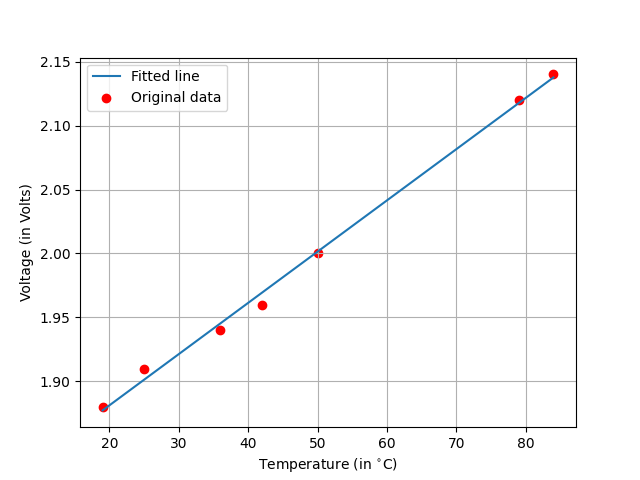
\includegraphics[width=\columnwidth]{figs/Train.png}
    \caption{Model Training}
    \label{fig:2}
\end{figure}

\newpage
\section{Model Evaluation}
The data used to evaluate the model is shown in the following table \ref{tab:2}.

\begin{table}[h]
    \centering
    %%%%%%%%%%%%%%%%%%%%%%%%%%%%%%%%%%%%%%%%%%%%%%%%%%%%%%%%%%%%%%%%%%%%%%
%%                                                                  %%
%%  This is a LaTeX2e table fragment exported from Gnumeric.        %%
%%                                                                  %%
%%%%%%%%%%%%%%%%%%%%%%%%%%%%%%%%%%%%%%%%%%%%%%%%%%%%%%%%%%%%%%%%%%%%%%

\begin{center}
\begin{tabular}{|c|c|}
\hline
\textbf{Voltage (in Volts)} & \textbf{Temperature (in $^{\circ}$C)} \\ \hline
1.68 & 25 \\ \hline
1.72 & 35\\ \hline
1.77 & 50 \\ \hline
\end{tabular}
\end{center}

    \caption{Test Data}
    \label{tab:2}
\end{table}

The test data, linear model curve are shown in the figure \ref{fig:3}.

\begin{figure}[ht]
    \centering
    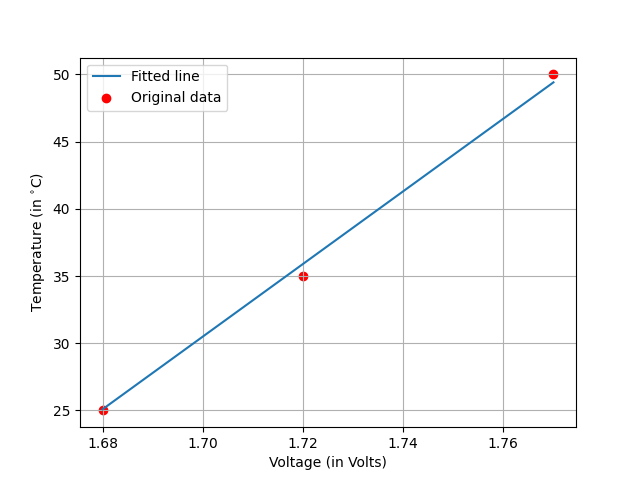
\includegraphics[width=\columnwidth]{figs/Test.png}
    \caption{Model Evaluation}
    \label{fig:3}
\end{figure}

\section{Conclusion}
In conclusion, this project effectively used machine learning to model the voltage-temperature characteristics of the PT-100, utilizing the least squares method and validating the model through test data. The project showcases the practical implementation of data collection and optimization using python.
\end{document}